\begin{ex}
 (Fuvest) Um tabuleiro tem 4 linhas e 4 colunas. O objetivo de um jogo é levar uma peça da casa inferior esquerda (casa (1, 1)) para a casa superior direita (casa (4, 4)), sendo que esta peça deve mover-se, de cada vez, para a casa imediatamente acima ou imediatamente à direita. Se apenas uma destas casas existir, a peça irá mover-se necessariamente para ela. Por exemplo, dois caminhos possíveis para completar o trajeto são:\newline $(1, 1)\rightarrow(1, 2)\rightarrow(2, 2)\rightarrow (2, 3)\rightarrow (3, 3)\rightarrow (3, 4)\rightarrow (4, 4)$\hspace{.4cm}e\hspace{.4cm} $(1, 1)\rightarrow (2, 1)\rightarrow (2, 2)\rightarrow (3, 2)\rightarrow (4, 2)\rightarrow (4, 3)\rightarrow (4, 4)$
 \begin{center}
     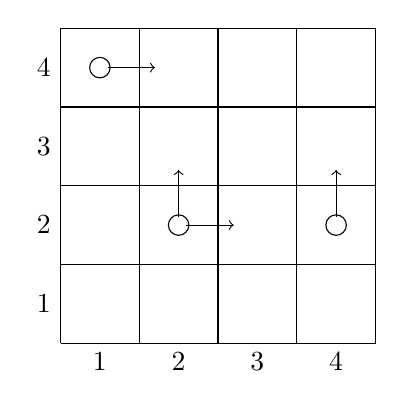
\begin{tikzpicture}
      \draw (0,0)--(4,0)--(4,4)--(0,4)--(0,0);\draw (1,0)--(1,4); \draw (2,0)--(2,4); \draw (3,0)--(3,4); \draw (0,1)--(4,1); \draw(0,2)--(4,2); \draw(0,3)--(4,3);
      \draw (1.5,1.5) circle[radius=.13];
      \draw[->](1.6,1.5)--(2.2,1.5);\draw [->](1.5,1.6)--(1.5,2.2);\draw[->](.6,3.5)--(1.2,3.5);
      \draw (.5,3.5) circle [radius=.13];
      \draw (3.5,1.5) circle [radius=.13];
      \draw[->](3.5,1.6)--(3.5,2.2);
      \node at (.5,0)[below]{1};\node at (1.5,0)[below]{2};
      \node at (2.5,0)[below]{3};\node at (3.5,0)[below]{4};
      \node at (0,.5)[left]{1};\node at (0,1.5)[left]{2};
      \node at (0,2.5)[left]{3};\node at (0,3.5)[left]{4};
     \end{tikzpicture}
 \end{center}
   \begin{enumerate}  [(a)]
       \item Por quantos caminhos distintos pode-se completar esse trajeto? 
       \item Suponha que o caminho a ser percorrido seja escolhido da seguinte forma: sempre que houver duas opções de movimento, lança-se uma moeda não viciada; se der cara, a peça move-se para a casa à direita e se der coroa, ela se move para a casa acima. Desta forma, cada caminho contado no item a) terá uma certa probabilidade de ser percorrido. Descreva os caminhos que têm maior probabilidade de serem percorridos e calcule essa probabilidade.
   \end{enumerate}
     \begin{sol}
     \phantom{A}
       \begin{enumerate} [(a)]
           \item para ir da casa (1,1) para a casa (4,4) é necessário ir 3 vezes para a direita e 3 vezes para cima (DDDCCC) $\Longrightarrow P^{3,3}_6 = \frac{6!}{3!3!}=20$
           \item maior probabilidade de ocorrer: CCCDDD ou DDDCCC $\Longrightarrow \frac{1}{2}\cdot\frac{1}{2}\cdot\frac{1}{2}\cdot1\cdot1\cdot1=\frac{1}{8}$
       \end{enumerate}
     \end{sol}
\end{ex}